\documentclass[12pt,a4paper]{article}

% Modele de rapport de stage et conseils de redaction, mise en page...
% L. Bellon, avril 2010

% definition des marges du document
\setlength{\topmargin}{0cm}
\setlength{\headheight}{0.4cm}
\setlength{\headsep}{0.8cm}
\setlength{\footskip}{1cm}
\setlength{\textwidth}{17cm}
\setlength{\textheight}{25cm}
\setlength{\voffset}{-1.5cm}
\setlength{\hoffset}{-0.5cm}
\setlength{\oddsidemargin}{0cm}
\setlength{\evensidemargin}{0cm}

% quelques package utiles
\usepackage{graphicx} % inclusion des figures
\usepackage{epstopdf} %inclusion .eps pour pdflatex

\usepackage{listings}
\usepackage{amsmath} % collection de symboles mathematiques
\usepackage{amssymb} % collection de symboles mathematiques

\usepackage{multicol,caption, subcaption}

\usepackage[utf8]{inputenc}
\usepackage[T1]{fontenc} % codage moderne des caracteres sous Latex

\usepackage[english]{babel}
\usepackage{natbib}

\usepackage{tabularx} % gestion avancee des tableaux

\usepackage{psfrag} % remplacement du texte d'une figure ps par du texte latex
\usepackage{siunitx} % units
\usepackage{physics} % to write physical equations

\usepackage{color} % gestion de differentes couleurs

\definecolor{linkcolor}{rgb}{0.3,0,0.2} % definition de la couleur des liens pdf
\usepackage[ pdftex,colorlinks=true,
pdfstartview=FitV,
linkcolor= linkcolor,
citecolor= linkcolor,
urlcolor= linkcolor,
hyperindex=true,
hyperfigures=false]
{hyperref} % fichiers pdf 'intelligents', avec des liens entre les references, etc.

\usepackage{fancyhdr} % entetes et pieds de pages personnalises

% commande de deplacement d'un objet
\newcommand{\drawat}[3]{\makebox[0pt][l]{\raisebox{#2}{\hspace*{#1}#3}}}

\usepackage{color}

\definecolor{mygreen}{rgb}{0,0.6,0}
\definecolor{mygray}{rgb}{0.5,0.5,0.5}
\definecolor{mymauve}{rgb}{0.58,0,0.82}

\lstset{ %
  backgroundcolor=\color{white},   % choose the background color; you must add \usepackage{color} or \usepackage{xcolor}
  basicstyle=\footnotesize,        % the size of the fonts that are used for the code
  breakatwhitespace=false,         % sets if automatic breaks should only happen at whitespace
  breaklines=true,                 % sets automatic line breaking
  captionpos=b,                    % sets the caption-position to bottom
  commentstyle=\color{mygreen},    % comment style
  deletekeywords={...},            % if you want to delete keywords from the given language
  escapeinside={\%*}{*)},          % if you want to add LaTeX within your code
  extendedchars=true,              % lets you use non-ASCII characters; for 8-bits encodings only, does not work with UTF-8
  frame=single,                    % adds a frame around the code
  keepspaces=true,                 % keeps spaces in text, useful for keeping indentation of code (possibly needs columns=flexible)
  keywordstyle=\color{blue},       % keyword style
  language=Octave,                 % the language of the code
  otherkeywords={*,...},            % if you want to add more keywords to the set
  numbers=left,                    % where to put the line-numbers; possible values are (none, left, right)
  numbersep=5pt,                   % how far the line-numbers are from the code
  numberstyle=\tiny\color{mygray}, % the style that is used for the line-numbers
  rulecolor=\color{black},         % if not set, the frame-color may be changed on line-breaks within not-black text (e.g. comments (green here))
  showspaces=false,                % show spaces everywhere adding particular underscores; it overrides 'showstringspaces'
  showstringspaces=false,          % underline spaces within strings only
  showtabs=false,                  % show tabs within strings adding particular underscores
  stepnumber=2,                    % the step between two line-numbers. If it's 1, each line will be numbered
  stringstyle=\color{mymauve},     % string literal style
  tabsize=2,                       % sets default tabsize to 2 spaces
  title=\lstname                   % show the filename of files included with \lstinputlisting; also try caption instead of title
}

\newcommand{\degree}{^{\circ}}
\newcommand{\cred}{\color{red}}

\graphicspath{{Figures/}} %Position of figures, pictures, etc

% definition de l'entete et du pied de page
\pagestyle{fancy}
\fancyhead[L]{\scriptsize \textsc{Field work: blabla TODO}}
\fancyhead[R]{\scriptsize \textsc{Romain Caneill}}
\fancyfoot[C]{ \thepage}

\begin{document}
% Pour faciliter la mise en forme de la page du titre, on supprime l'indentation automatique en debut de paragraphe
\setlength{\parindent}{0pt}

% Pas d'en-tete ni de pied pour la premiere page
\thispagestyle{empty}

\begin{minipage}{0.4\paperwidth}
  {\sc Physical Oceanography} \\
{\it Göteborgs universitet}\\
{\it Institutionen för marina vetenskaper}
\end{minipage}
\begin{minipage}{0.3\paperwidth}
  
\includegraphics[height=2.9cm]{gu}
\end{minipage}
\begin{minipage}{0.2\paperwidth}
  Romain Caneill\\
  PhD Student
\end{minipage}

\begin{center}
\vspace{.3cm}

\rule[5pt]{10cm}{0.5pt}
\vspace{10pt}

\textbf{\Large Find a title.}
\vspace{8pt}

\rule{10cm}{0.5pt}

\vspace{.3cm}

\parbox{15cm}{\small
\textbf{Abstract}: \it TODO
} %fin de la commande \parbox du resume

\vspace{0.5cm}

\parbox{15cm}{
\textbf{Keywords}: \it CTD, Field work, TODO
} %fin de la commande \parbox des mots clefs

\end{center}

\newpage

% Premiere page du rapport
\setcounter{page}{1}
\setlength\parindent{24pt}

\newpage

\tableofcontents

\newpage

\section{\label{sec_intro}Introduction}

TODO find references about fjords, skagerrak

\section{Materials and methods}
\subsection{Presentation of the field work and data acquisition}

field work 10-11 of December 2018

on board of 2 ships: Skagerrak and Trygve

\subsection{Data processing}
\subsubsection{Cleaning and calibration}
\paragraph{Reprocessing data, potential temp, absolute sal}
\paragraph{Gridding every meter 1-120 m depth}

\subsubsection{Data assimilation / creating new metrics}
\paragraph{Find some}
\paragraph{Turner angle TODO conpute}
\paragraph{Geostrophy TODO compute}
\paragraph{Profil fitting and layers}
Add a plot with the fit on a profile
\paragraph{No sub-mesoscale heat fluxes because no mixed layer}

\section{Results}

\paragraph{T-S diagram}
see figure \ref{fig:ts}

we recognize Skagerrak and Kattegat water \citep{bjork2003,gustafsson1996}

Kattegat salinity 15/20(depending on the source)-25

Skagerrak salinity between 33 (surface) to 35 (100m depth)

\begin{figure}
  \centering
  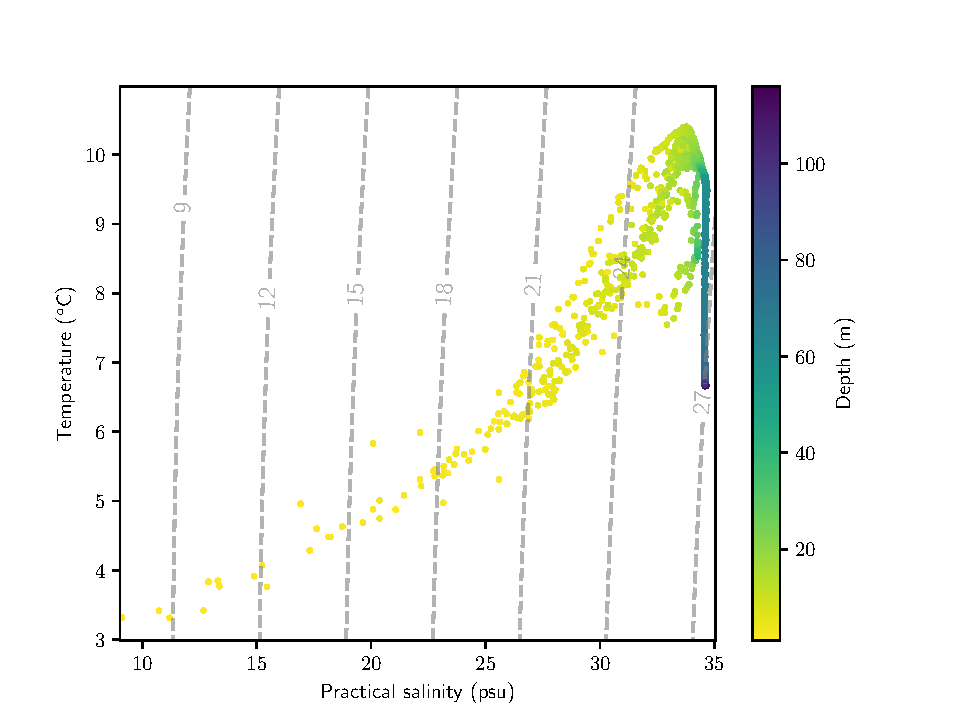
\includegraphics[width=.7\textwidth]{ts_conv}
  \caption{\label{fig:ts}T-S diagram}
\end{figure}

\paragraph{warm water layer}
warm water in the fjord, see mean depth, std depth, mean T and S, see spatial
distribution

\paragraph{strong halocline}

\paragraph{Turner angle}
What is happening here?

\paragraph{Geostrophy}
What is happening here?

\paragraph{Upwelling event? Mixing?}
\citep{arneborg2003}

\section{Discussion}

TODO

\section{Conclusion}

See what is the context\\
What we did\\
What we showed/saw\\
What is the conclusion

%\newpage

\bibliographystyle{../Biblio/agufull08}
\bibliography{../Biblio/biblio}

\newpage

%\renewcommand\thefigure{\thesection.\arabic{figure}}
\appendix
\setcounter{figure}{0}

TODO

ALL THE FIGURES I WANT TO PUT ON THE REPORT

For all profiles, put 2 different color for offshore and fjord
\begin{figure}
  \centering
  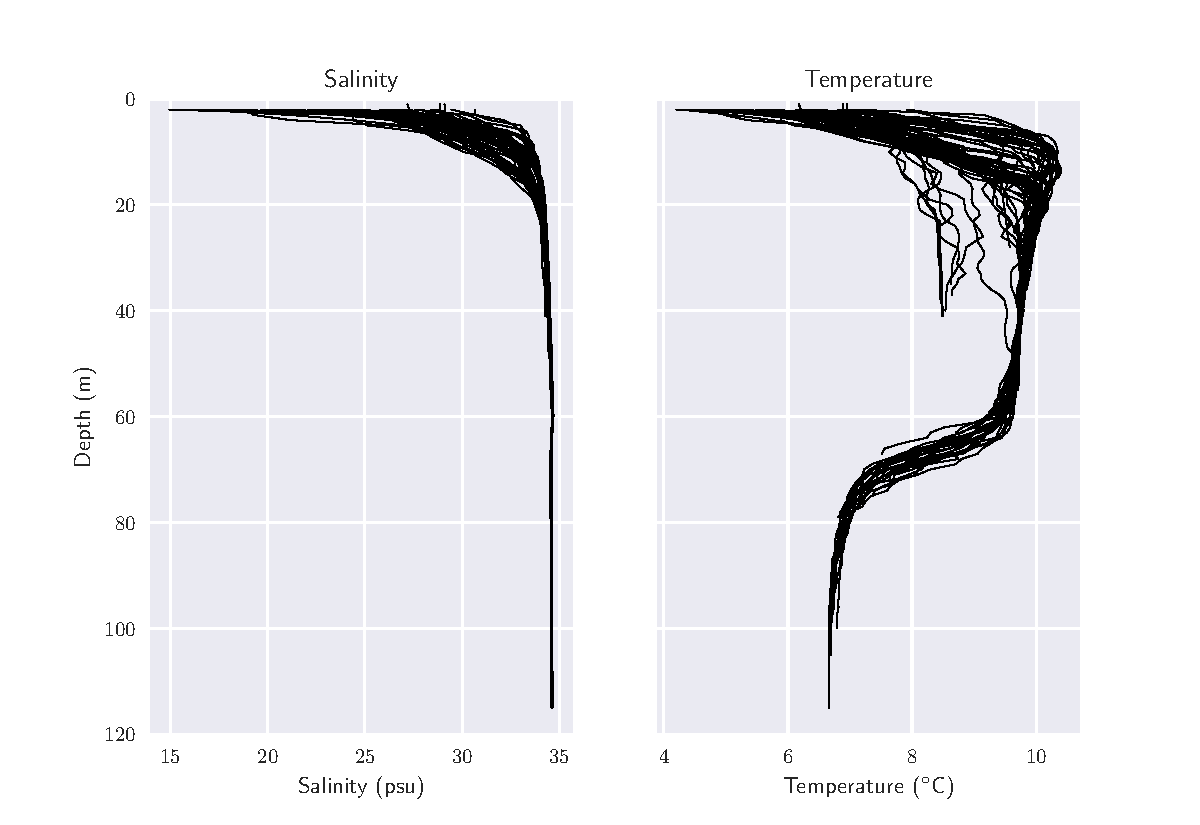
\includegraphics[width=.3\textwidth]{profileTot}
  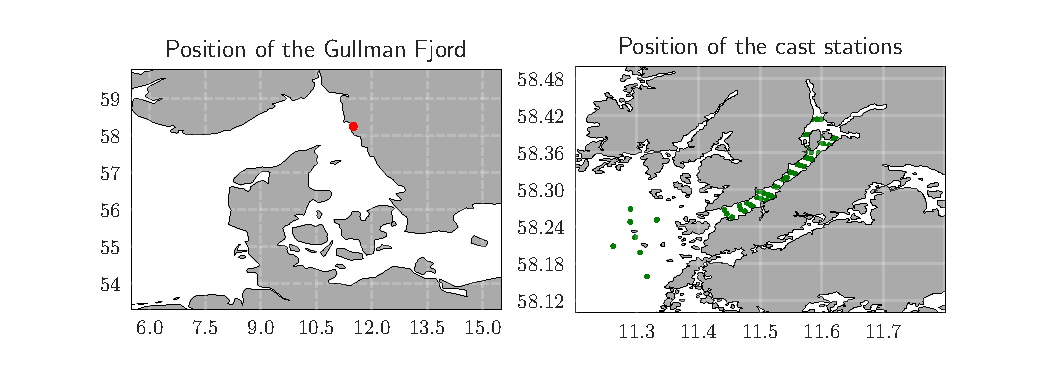
\includegraphics[width=.3\textwidth]{stations}
  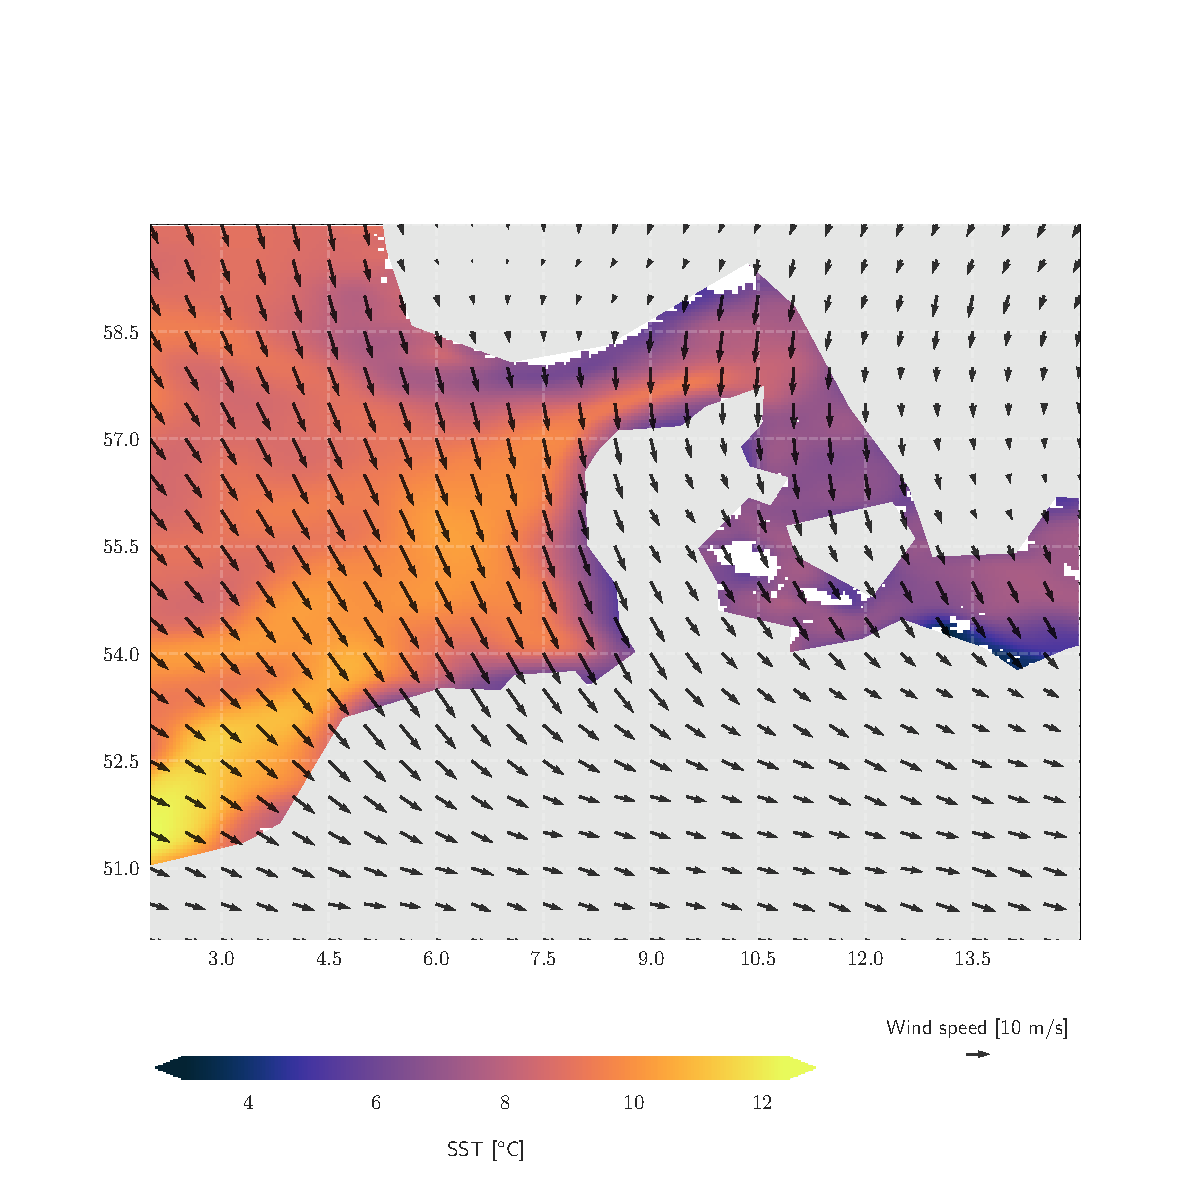
\includegraphics[width=.3\textwidth]{synoptic_conditions}
  \includegraphics[width=.3\textwidth]{{sal_20181210}}
  \includegraphics[width=.3\textwidth]{{layer_bottom_of_thermocline}}
  \includegraphics[width=.3\textwidth]{{layer_bottom_of_warm_water}}
  \includegraphics[width=.3\textwidth]{{transect_0}}
  \includegraphics[width=.3\textwidth]{{transect_2}}
\end{figure}

\end{document}
